\documentclass[11pt, a4paper]{article}
\usepackage{soul, color, xcolor}
\usepackage{graphicx,float,subcaption,caption} % Required for inserting images
\usepackage{ctex,geometry}
\usepackage{bm,amsmath}
\geometry{left = 2.54cm, right = 2.54cm, top = 3.18cm, bottom = 3.18cm}
\begin{document}
\setcounter{page}{0}
\newpage
\pagenumbering{Roman}
\setcounter{page}{1}
\tableofcontents
\newpage
\setcounter{page}{1}
\pagenumbering{arabic}
\section{The Electric Field}
\subsection{Coulomb’s Law}
$$\vec{F} = k\frac{q_1q_2}{r^2} \hat{r} = \frac{1}{4\pi \epsilon_0}\frac{q_1q_2}{r^2} \hat{r}$$
$k = 8.99\time 10^9$, permittivity constant $\xi_0 = 8.85\times10^{-12}$

\subsection{Gauss's Law}
$\vec{A}$ pointing outward from the surface. An inward piercing field is
negative flux. An outward piercing field is positive flux. 
The integral form:
$$\epsilon_0\oint\vec{E}\cdot d\vec{A}=q_{\mathrm{enc}}$$
If qenc is positive, the net flux is outward; if qenc is
negative, the net flux is inward.
The deriavative form:
$$\nabla \cdot \vec{E} = \frac{\rho}{\epsilon}$$

The electric field due to a charge outside the
Gaussian surface contributes zero net flux through the
surface, because as many field lines due to that charge
enter the surface as leave it.
\subsection{The way to find the Electric field}
\textbf{利用库仑定律力的合成叠加原理求场强}

1. Ring superposition 
\begin{figure}[htbp]
    \centering
    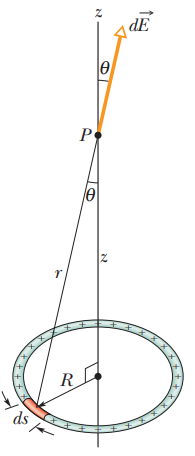
\includegraphics[height = 4cm]{2.png}
\end{figure}
$$\frac{qz}{4\pi\epsilon_0(z^2+R^2)^{3/2}},$$
2. Disk superposition 
\begin{figure}[htbp]
    \centering
    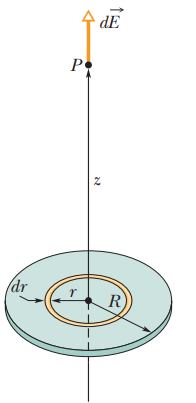
\includegraphics[height = 4cm]{3.png}
\end{figure}
$$\frac\sigma{2\epsilon_0}\left[1-\frac z{(z^2+R^2)^{1/2}}\right]$$
\textbf{利用高斯定理求场强}

1.Spherical Symmetry: Inside and outside a uniform sphere of charge
\begin{figure}[htbp]
    \centering
    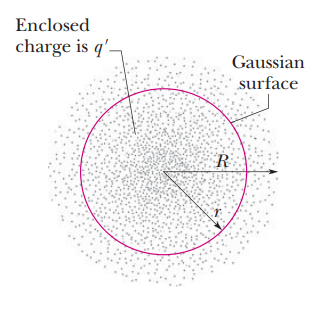
\includegraphics[height = 4cm]{4.png}
\end{figure}
$$\begin{cases}
    &\vec{E}=\left(\frac q{4\pi\epsilon_0R^3}\right)\vec{r} ,\qquad r \le R \\
    &\vec{E} = \left(\frac q{4\pi\epsilon_0r^3}\right)\vec{r},\qquad r > R 
\end{cases}$$

2.Planar Symmetry:An infinite sheet with a uniform surface charge density $\sigma$.
\begin{figure}[htbp]
    \centering
    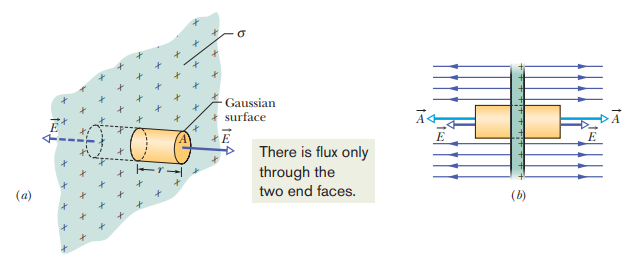
\includegraphics[height = 4cm]{5.png}
\end{figure}
$$E = \frac{\sigma}{2\epsilon_0}$$  
 This result holds for any point at a finite distance from the sheet.

3.Cylindrical Symmetry:An infinite line of charge with a uniform line density $\lambda$.
\begin{figure}[htbp]
    \centering
    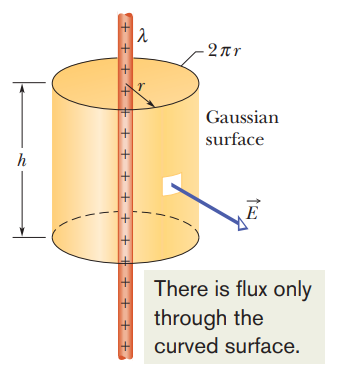
\includegraphics[height = 4cm]{6.png}
\end{figure}
$$E=\frac{\lambda h}{\epsilon_0(2\pi rh)}=\frac\lambda{2\pi\epsilon_0r}$$

\textbf{利用电势求场强}

$$E_x=-\frac{\partial V}{\partial x};\quad E_y=-\frac{\partial V}{\partial y};\quad E_z=-\frac{\partial V}{\partial z}$$
\section{Electric Potential}

\begin{align*}
    &V = \frac{-W}{q} = \frac{U}{q}\\
    &V_f- V_i = -\int_i^F \vec{E}\cdot\mathrm{d}\vec{s} \rightarrow V = -\int_{infinity}^{\vec{r}}\vec{E}\cdot\vec{S} = \frac{1}{4\pi \epsilon_0}\frac{q}{r}\\
    &\text{net potential: }V=\sum_{i=1}^nV_i=\frac1{4\pi\epsilon_0}\sum_{i=1}^n\frac{q_i}{r_i}
\end{align*}

The total potential energy of  systems of charged particles:
$$U_{\mathrm{tot}}=\sum_{i<j}U_{ij}=\frac1{4\pi\epsilon_0}\sum_{i<j}\frac{q_iq_j}{r_{ij}}= \frac1{8\pi\epsilon_0}\sum_{i\ne j}\frac{q_iq_j}{r_{ij}}$$

\textbf{Summary}

\begin{itemize}
    \item A charged particle: $$\frac{1}{4\pi \epsilon_0}\frac{q}{r}$$
    \item An electric dipole: $$\frac1{4\pi\epsilon_0}\frac{p\cos\theta}{r^2}$$
    \item A continuous charge distribution (e.g., rod and disk): $$V=\frac1{4\pi\epsilon_0}\int\frac{dq}r$$
    \item Electric potential energy of a system of charged particles: $$U_{\mathrm{tot}}=\sum_{i<j}U_{ij}=\frac1{4\pi\epsilon_0}\sum_{i<j}\frac{q_iq_j}{r_{ij}}$$
\end{itemize}

\section{Electric Dipole}
Electric dipole moment: $$\vec{p} = q\vec{d}$$
\begin{figure}[htbp]
    \centering
    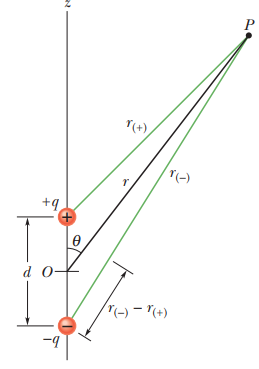
\includegraphics[height = 4cm]{7.png}
\end{figure}

The electric field at \underline{an arbitrary point P along the dipole axis}, at distance $z$ from the dipole’s center,
$$E=\frac q{4\pi\epsilon_0(z-\frac12d)^2}-\frac q{4\pi\epsilon_0(z+\frac12d)^2}$$

$$\Longrightarrow E=\frac1{2\pi\epsilon_0}\frac p{z^3} \qquad(z \gg d)$$

The net torque when a dipole in a uniform electric field:

$$\tau=-Fd\sin\theta=-pEsin\theta = \vec{p}\times \vec{E}$$

Potential due to an Electric Dipole:
$$V=\frac1{4\pi\epsilon_0}\frac{p\cos\theta}{r^2}=\frac1{4\pi\epsilon_0}\frac{\vec{p}\cdot\vec{r}}{r^3}\qquad(r\gg d)$$


\section{The Triangle of Electrostatics}

\begin{figure}[htbp]
    \centering
    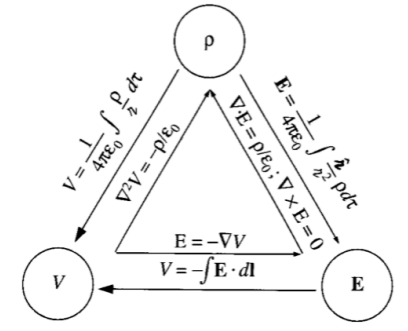
\includegraphics[height = 4cm]{8.png}
\end{figure}

\section{The Electrical Properties of Conductors}
\subsection{A Charged Isolated Conductor}
Electrostatic Equilibrium: 
$$\boxed{\vec{E}_{inside} = 0,\quad q_{net}^{inside} = 0,\quad V_{inside} = V_{surface}}$$

1. All points of the conductor – whether on the surface or
inside – come to the same potential(even if the conductor has an internal cavity
and even if that cavity contains a net charge).

2. All the excess charge remains on the outer surface of the conductor(even if the conductor has an internal cavity).

\subsubsection{Electric Field Outside Isolated Conductors}
Notice that the surface charge density $\sigma$ varies, however, over the
surface of any \underline{nonspherical conductor}.

Direction: The electric field $\vec{E}$ at and just outside the conductor’s surface must also be
perpendicular to that surface.

Cylindrical Gaussian surface: 
\begin{figure}[htbp]
    \centering
    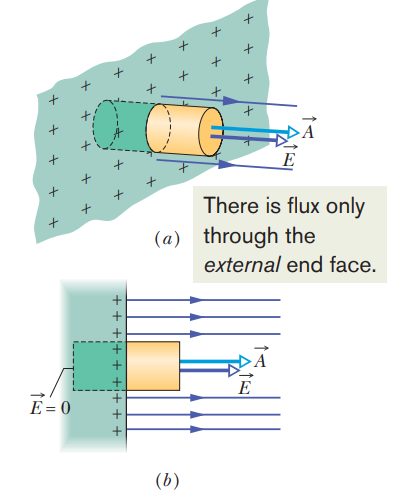
\includegraphics[height = 4cm]{9.png}
\end{figure}
$$\begin{aligned}
    &\epsilon_0EA = \sigma A\\
    \Rightarrow& \vec{E} = \frac{\sigma}{\epsilon_0}\hat{n} 
\end{aligned}$$

\subsubsection{Parallel Plates}
\begin{itemize}
    \item Single Plate: all the excess charge spreads out on the
    two faces of the plate with a uniform surface charge density.
    \item Two Parallel Plates: all the excess charge moves onto the inner faces of the plates.
\end{itemize}

\subsection{Charge Inside a Spherical Metal Shell}
\begin{figure}[htbp]
    \centering
    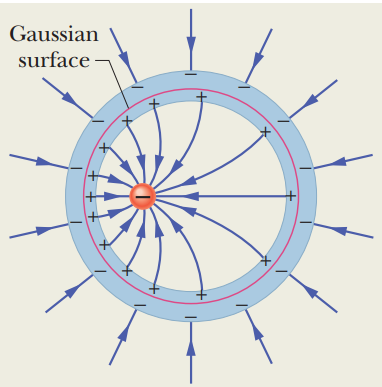
\includegraphics[height = 4cm]{10.png}
\end{figure}
Charge distribution: a total charge $Q$ must lie on the inner wall of
the shell,  and a total $-Q$ move to the outer wall and they must \underline{spread out uniformly}.

\subsection{Charge Above a Infinite Grounded Gonducting Plane}

\textbf{The Method of Image}
\begin{figure}[htbp]
    \centering
    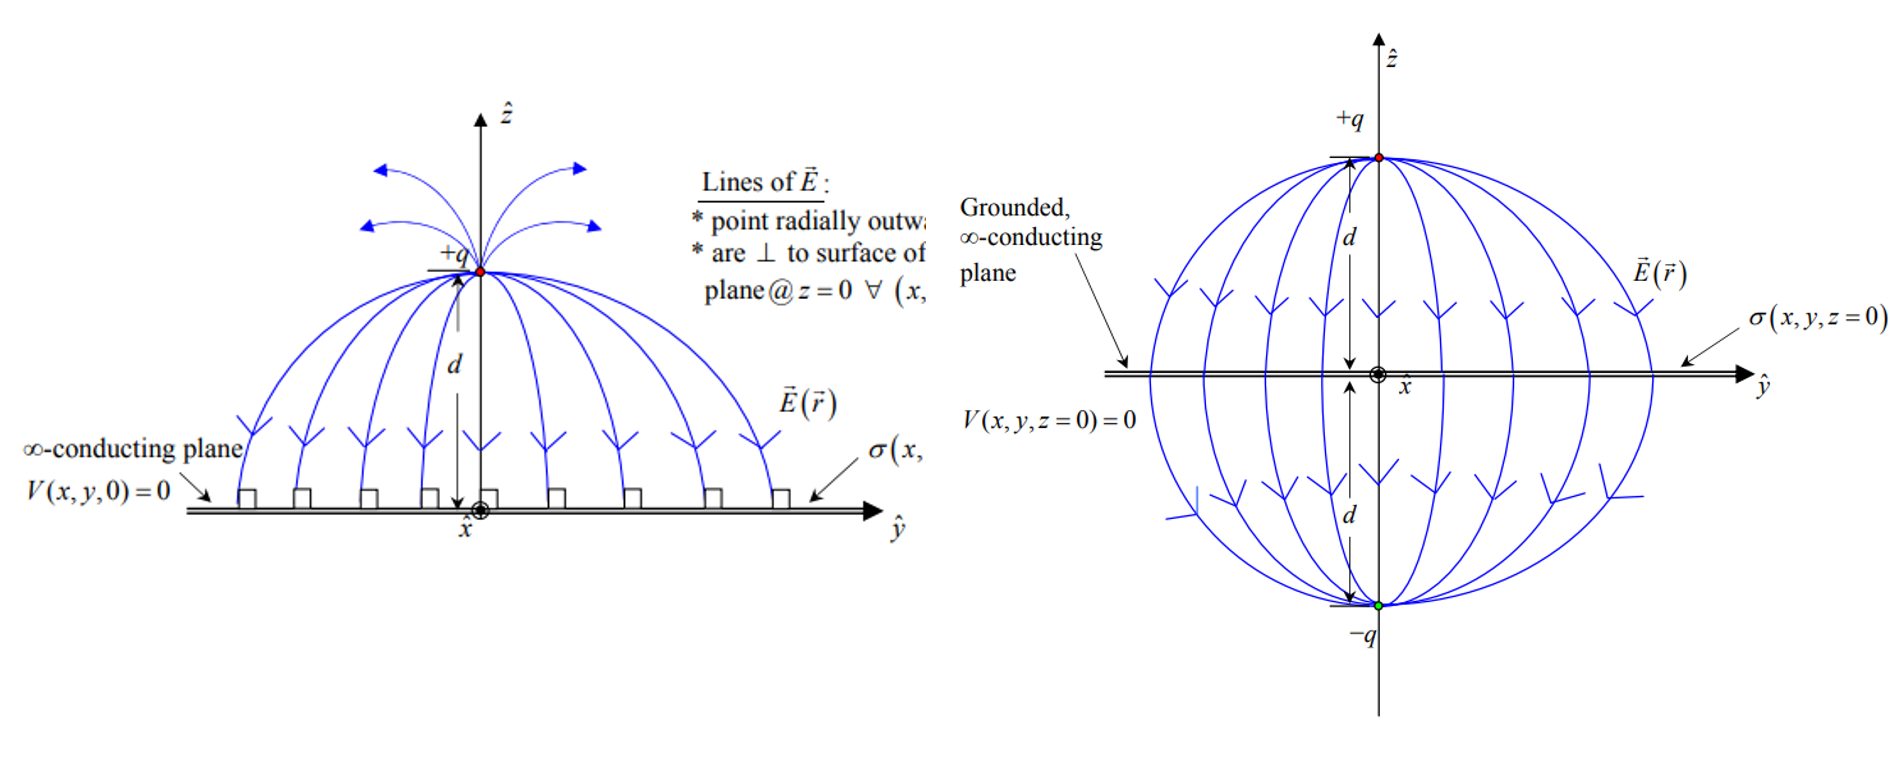
\includegraphics[height = 4cm]{11.png}
\end{figure}
$$V=\frac{q/4\pi\epsilon_0}{\sqrt{x^2+y^2+(z-d)^2}}-\frac{q/4\pi\epsilon_0}{\sqrt{x^2+y^2+(z+d)^2}}.$$
$$\sigma=-\epsilon_0\left.\frac{\partial V}{\partial z}\right|_{z=0}=-\frac{qd}{2\pi(x^2+y^2+d^2)^{3/2}}.$$
The total charge induced on the z = 0 plane is $-q$.
\section{Resistance and Capacitance}
\subsection{Resistance}
\indent \textbf{Concepts}\\
\begin{itemize}
    \item Current Density: $$i =\int \vec{J}d\vec{A}$$ 
    \item 
\end{itemize}
$\bullet$ 
$\bullet$ Drift Velocity : ($n$ is the number of carriers per unit volume) $$i = nAev_d \qquad \vec{J} = ne\vec{v_d}$$ \\
$\bullet$ Resitivity and conducticivity: 

1. $$\vec{E} = \rho \vec{J} \Rightarrow \rho = \frac{1}{\sigma} = \frac{E}{J} $$

2. $$\vec{a} = -\frac{e\vec{E}}{m}$$

In the average time $\tau$(mean free time) between collisions, the electro will on average acquire

$$\begin{aligned}
    &\vec{v}_d = \vec{a}\tau = -\frac{e\vec{E}}{m}\tau
    &\Rightarrow \boxed{\rho= \frac{m}{ne^2 \tau}}
\end{aligned}$$
\indent $\bullet$ Resistance:$$R=  \frac{V}{i}\quad R = \rho\frac{L}{A}$$

\textbf{Equation of Continuity} $$\frac{\partial \rho}{\partial t} = \nabla \cdot \vec{J}$$ 

\subsection{Calculating Capacitance}
\begin{figure}[htbp]
    \centering
    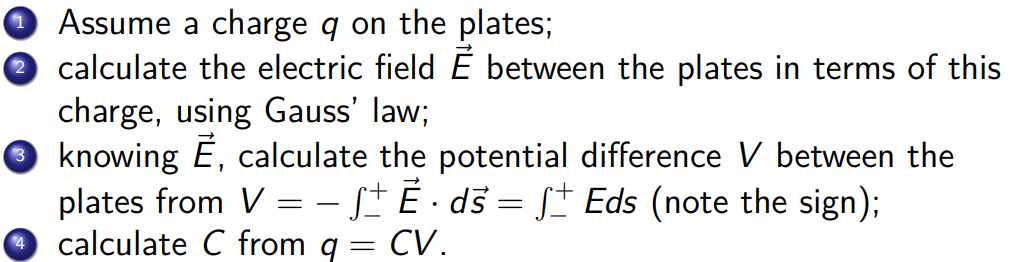
\includegraphics[height = 3cm]{12.png}
\end{figure}


\textbf{Capacitance of a Parallel-Plate Capacitor:}
\begin{figure}[htbp]
    \centering
    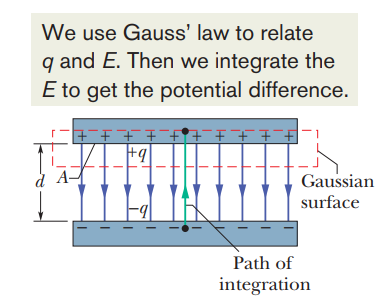
\includegraphics[height = 4cm]{13.png}
\end{figure}
$$\begin{aligned}
    &q = \epsilon_0EA\\
    &C = \frac{\epsilon_0 A}{d}
\end{aligned}$$

\textbf{Capacitance of a Cylindrical Capacitor:}
\begin{figure}[htbp]
    \centering
    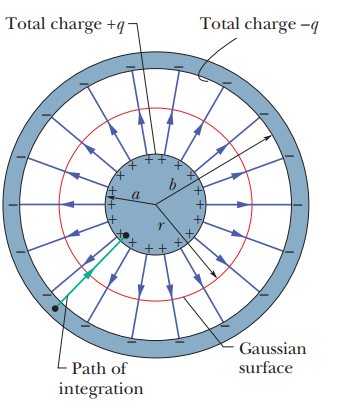
\includegraphics[height = 4cm]{14.png}
\end{figure}
$$\begin{aligned}
    &q=\epsilon_0EA=\epsilon_0E(2\pi rL)\\
    &V=-\int_{-}^{+}\vec{E}\cdot d\vec{s}=-\frac q{2\pi\epsilon_0L}\int_{b}^{a}\frac{dr}r=\frac q{2\pi\epsilon_0L}\ln\left(\frac ba\right)\\
    &C=\frac qV=2\pi\epsilon_0\frac L{\ln(b/a)}
\end{aligned}$$

\subsection{Energy Stored in a Capacitor}
Energy:$$U=\frac{q^2}{2C}=\frac12CV^2$$

Energy Density:
$$u=\frac12\epsilon_0E^2$$

Gauss' law with a dielectric (with$\vec{D}\equiv\kappa\epsilon_0\vec{E}$)
$$\oint\vec{D}\cdot d\vec{A}=\epsilon_0\oint\kappa\vec{E}\cdot d\vec{A}=q$$
\subsection{DC Circuits}
\textbf{Concepts}
emf $\varepsilon$, pover $P$, dielectric constant $\kappa$, electric displacement $\vec{D}$

$$
\begin{aligned}\mathcal{E}&=\frac Wq\\P&=iV\\P&=i^2R=\frac{V^2}R\end{aligned}
$$

\textbf{Kirchhoff ’s loop rule:} The algebraic sum of the changes in
potential encountered in a complete traversal of any loop of a circuit must be zero.

\textbf{Charging a Capacitor}
$$\begin{gathered}
    \frac{dU}{dt}=\frac qC\frac{dq}{dt}=iE-i^2R. \\
    \bullet\text{ Noting }i=dq/dt\text{,we find} \\
    R\frac{dq}{dt}+\frac qC=\varepsilon, \\
    \text{capacitive time constant} \tau = RC\\
    \Rightarrow q = C\varepsilon(1-e^{-t/\tau})
    \Rightarrow i = \frac{\varepsilon}{R}e^{-t/\tau}
\end{gathered}$$

\textbf{Discharging a Capacitor}
Energy change:
$$\begin{aligned}&\frac d{dt}\left(\frac{q^2}{2C}\right) + i^2R = 0\\
    &\frac{dq}{dt} + \frac{q}{RC} = 0\end{aligned}\\$$
这个方程也可以从Loop Rule列回路电压变化为0,电压降等于电压升。
\subsection{Dielectrics and Gauss’ Law}    
$$\epsilon_0\oint\kappa\vec{E}\cdot d\vec{A}=\oint\vec{D}\cdot d\vec{A}=q,$$
electric displacement $\vec{D} \equiv \kappa\epsilon \vec{E}$

\section{The Ampere Force}
$$\vec{F}_B = q\vec{v}\times \vec{B}$$
利用右手确定方向

\subsection{Hlical Movement}
The radius of the helix: $r=\frac{mv_\perp}{|q|B}$.\\
The parallel component $v_{||}$ determines the pitch p of the 
helix – that is, the distance between adjacent turns.

\subsection{The Hall Effect}
$$\begin{aligned} &i = JA =nev_dA\\
    &eE = ev_dB_z\\
    &V = Ed = -v_dBd = -\frac{i}{neA}Bd = -\frac{B}{ne}Jd\\
    &\text{Hall resistivity and coefficient} \rho_{xy}=\frac{E_y}{J_x}=-\frac B{ne},\quad R_H=\frac{E_y}{B_zJ_x}=-\frac1{ne}\\
\end{aligned}$$

\begin{figure}[htbp]
    \centering
    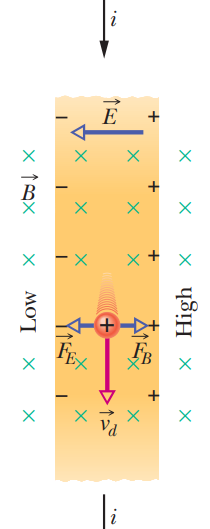
\includegraphics[height = 5cm]{Hall Effect.png}
\end{figure}

\subsection{Current-Carrying Wire}
$$\begin{aligned}
    &\vec{F} = i\vec{L} \times \vec{B}\\
    &\mathrm{d}\vec{F} = i \mathrm{d}\vec{L}\times \vec{B}\\
\end{aligned}$$

\section{The Magenetic Field}
\subsection{Biot-Savart law}
$$d\vec{B}=\frac{\mu_0}{4\pi}\frac{id\vec{s}\times\vec{r}}{r^3},$$
where the constant $µ0 = 4π × 10^{−7} T · m/A$ is called the permeability constant.
\begin{figure}[htbp]
    \centering
    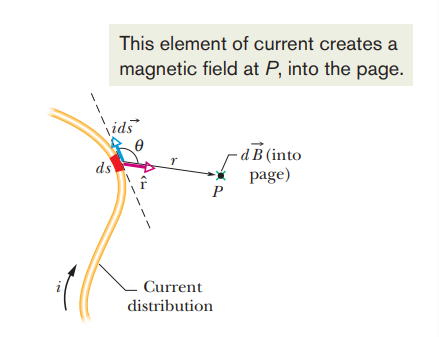
\includegraphics[width = 5cm]{Biot-Savart Law.png}
    \caption{Biot-Savart Law}
\end{figure}
\textbf{Force Between Two Parallel Wires}
\begin{figure}[htbp]
    \centering
    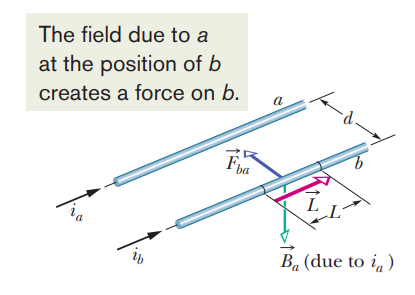
\includegraphics[width = 5cm]{Two Parallel Wires.png}
    \caption{Force Between Two Parallel Wires}
\end{figure}
$F_{ba}=|i_b\vec{L}\times\vec{B}_a|=\frac{\mu_0Li_ai_b}{2\pi d},$

\subsection{Ampere's Law}
\begin{figure}[htbp]
    \centering
    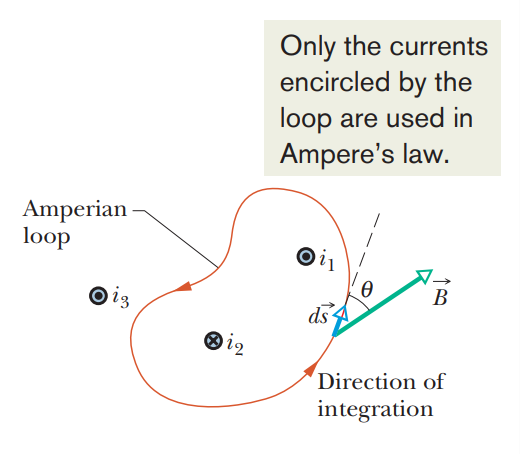
\includegraphics[width = 5cm]{Amprerian Loop.png}
    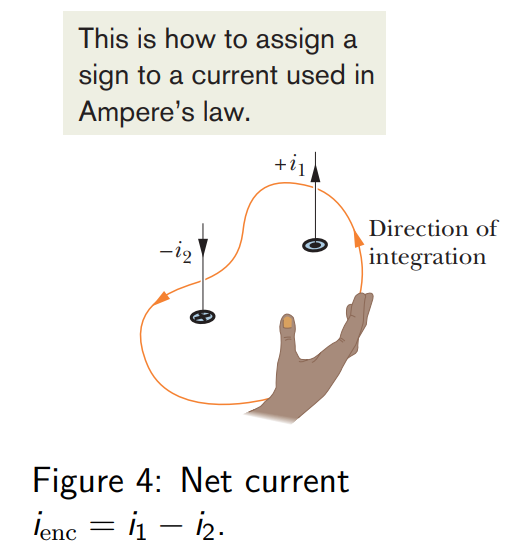
\includegraphics[width = 5cm]{net current sign.png}
\end{figure}
$$\oint\vec{B}\cdot d\vec{s}=\mu_0i_{\mathrm{enc}},$$
where $i_{enc}$ is the net current encircled by the closed loop.

\subsection{Examples}
\subsubsection{ A Long Straight Wire}
\begin{figure}[htbp]
    \centering
    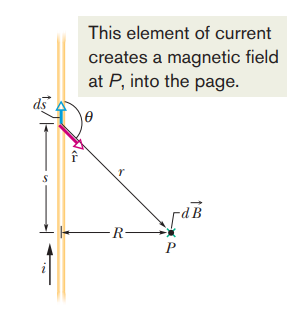
\includegraphics[width = 4cm]{Long straight wire .png}
    \caption{A Long Straight Wire}
\end{figure}

$$\begin{aligned}
    d \vec{B}& =\frac{\mu_0}{4\pi}\frac{id\vec{s}\times\vec{r}}{r^3}  \\
    &=\frac{\mu_0}{4\pi}\frac{id\vec{s}\times\vec{R}}{r^3}.
\end{aligned}$$
$$B=\frac{\mu_0}{4\pi}\int_{-\infty}^\infty\frac{iRds}{r^3}=\frac{\mu_0i}{4\pi R}\left[\int_{-\infty}^\infty\frac{R^2ds}{r^3}\right],$$    
$$B=\frac{\mu_0i}{2\pi R},$$
The direction follows a curled-straight right-hand rule(右手螺旋法则).

\subsubsection{Outside a Long Straight Wire}
$$\oint\vec{B}\cdot \mathrm{d}\vec{S} = B(2\pi r) = \mu_0 i \Rightarrow boxed{B = \frac{\mu_0 i}{2\pi r}}$$
\subsubsection{Inside a Long Straight Wire}
Supposed that the current is \underline{uniformly distributed over the\\
cross section of the wire},
$$\begin{aligned}
    &i_{enc} = \frac{r^2}{R^2}\\
    &B = \frac{\mu_0 i_{end}}{2\pi r} = \frac{\mu_0}{2\pi R^2}r
\end{aligned}$$

\subsubsection{A Sheet Of Moving Charge}
Consider an infinite flat sheet of current density $J_s$
in the y-direction:
\begin{figure}
    \centering
    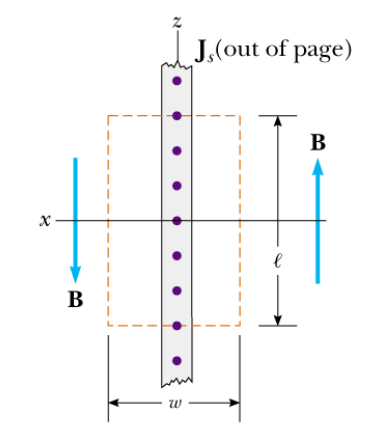
\includegraphics[width = 5cm]{Sheet of Moving Charge.png}
    \caption{An infinite Sheet}
\end{figure}
Ampere’s law can be applied to the
rectangular path:
$$\begin{aligned}&\oint\vec{B}\cdot d\vec{s}=2B\ell=\mu_0(J_s\ell)\\
&B = \frac{\mu_0 J_s}{2}\end{aligned}$$

\subsubsection{Magnetic Field of a Solenoid}
The field inside the coil is uniform and parallel
to the solenoid axis. The magnetic field outside the
solenoid is zero.
\begin{figure}[htbp]
    \centering
    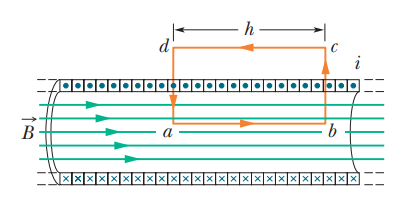
\includegraphics[width = 5cm]{Solenoid.png}
    \caption{Amperian Loop of Solenoid}
\end{figure}

$$\begin{aligned}
    \oint\vec{B}\cdot d\vec{s} &= \int_{a}^b \vec{B} \cdot \mathrm{d}\vec{s} &= Bh
\end{aligned}$$
Let $n$ be \underline{the number of turns per unit length of thesolenoid}; 
then the loop encloses nh turns and:
$$i_{enc}= i(nh)$$
$$\Rightarrow B = \mu_0 in$$
\subsubsection{Magnetic Field of a Toroid}
A toroid is a solenoid that has been curved until its two
ends meet, forming a hollow donut.
\begin{figure}[htbp]
    \centering
    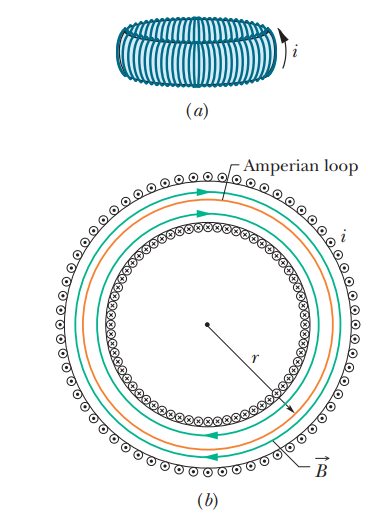
\includegraphics[width = 5cm]{Toroid.png}
    \caption{Amperian Loop of Toroid}
\end{figure}
$$B = \mu_0 i\frac{N}{2\pi r}$$
B = 0 for points outside an ideal toroid.
\subsection{The Properties of B}
\begin{itemize}
    \item The curl of $\vec{B}$: (安培定律的微分形式) $$\begin{aligned}
        &\int_S(\nabla\times\vec{B})\cdot d\vec{A}=\oint\vec{B}\cdot d\vec{s}=\mu_0i_{\mathrm{enc}}=\mu_0\int_S\vec{J}\cdot d\vec{A},\\
        &\nabla\times\vec{B} = \mu_0 \vec{J}(\vec{r})
    \end{aligned}$$
    \item The Divergence of $\vec{B}$:(高斯定理的微分形式)$$\begin{aligned}
        &\oint\vec{B}\cdot d\vec{A}=\int(\nabla\cdot\vec{B})dV=0.\\
        & \nabla\cdot\vec{B} = 0
    \end{aligned}$$
\end{itemize}

\section{Magnetic Properties of Materials}
\subsection{Magenetic Dipole}
\textbf{The total torque on the coil}:
$$\vec{\tau}=Ni\vec{A}\times\vec{B}=\vec{\mu}\times\vec{B},$$
where $\vec{\mu} = Ni\vec{A}$ is known as the magnetic dipole
moment of the coil.

\begin{figure}[htbp]
    \centering
    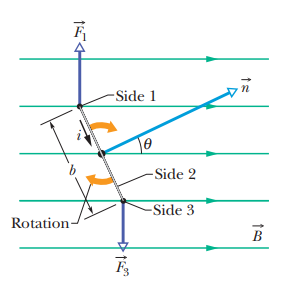
\includegraphics[width = 5cm]{Megenetic Dipole.png}
\end{figure}

$$\tau=-\mu B\sin\theta=-\frac\partial{\partial\theta}(-\mu B\cos\theta).$$
\textbf{The energy of a magenetic dipole:}
$$U_B = -\vec{mu} \cdot \vec{B} = -\mu B \cos \theta$$
\textbf{The field of a Megnetic Dipole}
The Megneticat field at the center of a single-loop coil with a magnetic dipole moment $µ$
$$B = \frac{\mu_0}{2\pi}\frac{\mu}{R^3}$$
The magnetic field at an axial point:

\subsection{Magnetic Materials}
\begin{figure}[htbp]
    \centering
    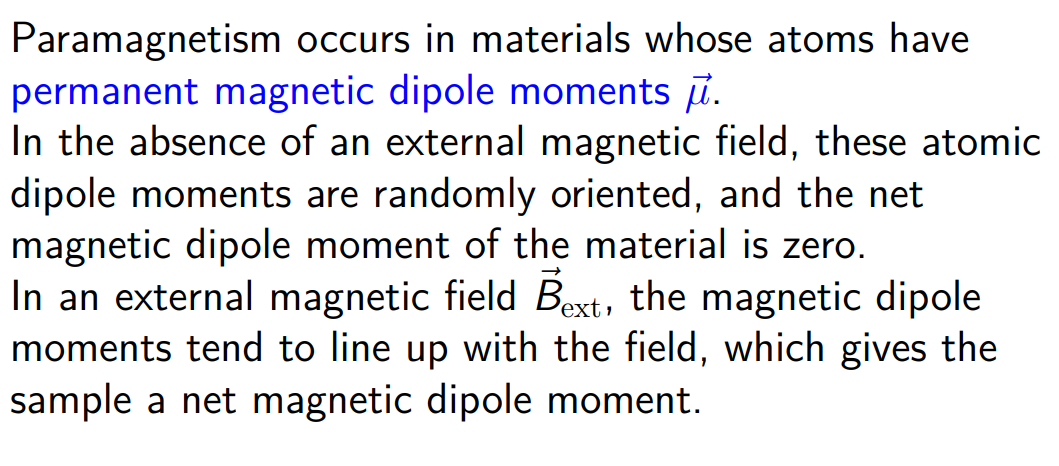
\includegraphics[height = 4cm]{paramagnetism0.png}
    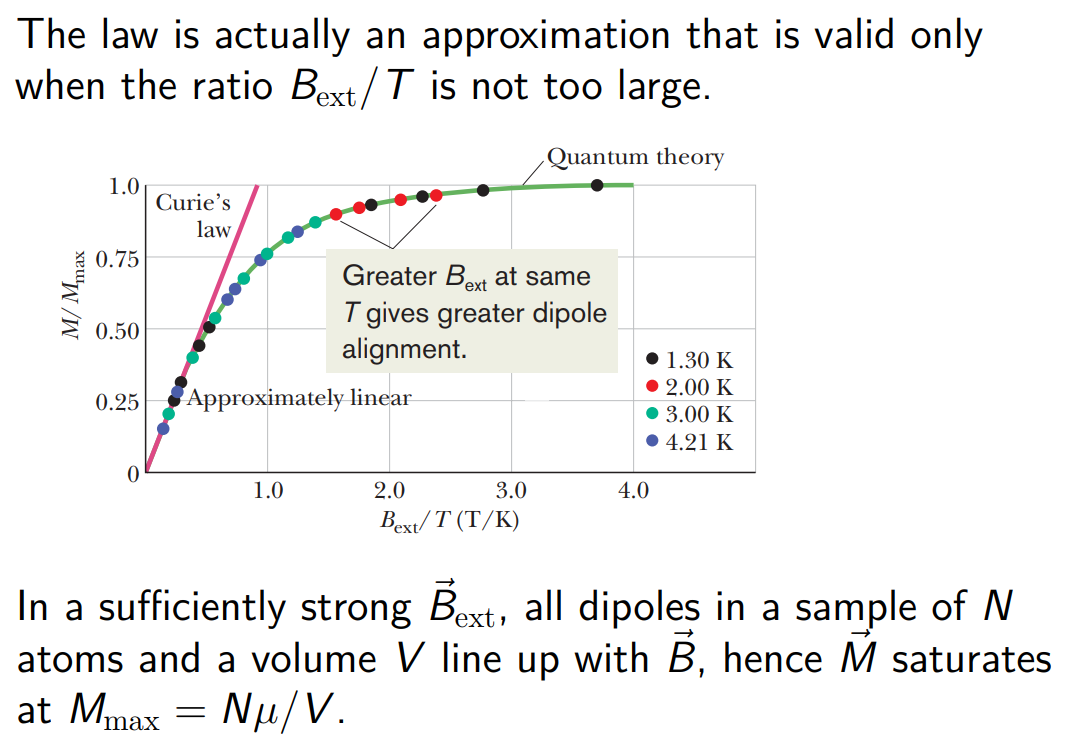
\includegraphics[height = 4cm]{paramagnetism1.png}
    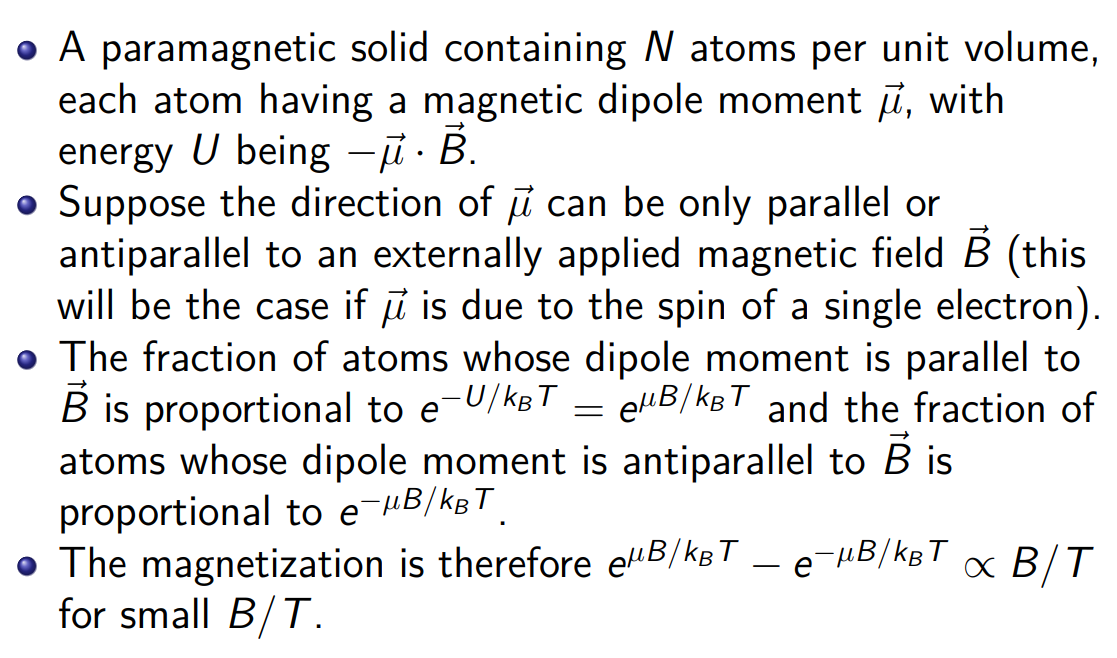
\includegraphics[height = 4cm]{paramagnetic3.png}
\end{figure}

\section{Faraday’s Law of Induction}
$$\mathcal{E}=-N\frac{d\Phi_B}{dt}.$$
积分形式:
$$\oint\vec{E}\cdot d\vec{s}=-\frac d{dt}\int\vec{B}\cdot d\vec{A}$$
微分形式:
$$\nabla\times\vec{E}=-\frac{\partial\vec{B}}{\partial t},$$
Notice  electric potential has no meaning for electric fields that are
produced by induction.
\section{Inductors and Inductance}
$$L=N\Phi_B/i$$ 
for a solenoid, $$L = \mu_0 n^2 $$
\subsection{RL Circuits}
Loop Rule:
$$L\frac{di}{dt}+Ri=\varepsilon$$
inductive time constant: $\tau_L = \frac{L}{R}$
$$i= \frac{\varepsilon}{R}(1-e^{-t/\tau_L})$$
\subsection{Energy and Energy Density}
$$U_B = \frac{1}{2}LI^2$$
$$u_b = \frac{B^2}{2\mu_0}$$
\subsection{Mutual Induction}
Self-inductance L (of a single circuit) and
mutual inductance M12 = M21 (of two circuits)
$$\begin{gathered}
    \mathcal{E}_{11}=-\frac{d(N_1\Phi_{11})}{dt}=-L_1\frac{di_1}{dt} \\
    \mathcal{E}_{21}=-\frac{d(N_2\Phi_{21})}{dt}=-M_{21}\frac{di_1}{dt} 
    \end{gathered}$$
\section{AC Circuits}
\subsection{LC Oscillations}
The total energy $U$ in an oscillating $LC$ circuit is given by
$$
U=U_B+U_E=\frac{\mathrm{Li}^2}2+\frac{q^2}{2C}.
$$
In the absence of resistance, $U$ remains constant with time
$$
\frac{dU}{dt}=\frac d{dt}\left(\frac{Li^2}2+\frac{q^2}{2C}\right)=Li\frac{di}{dt}+\frac qC\frac{dq}{dt}=0.
$$
With $i=dq/dt$ and $di/dt=d^2q/dt^2$, we find 
$$\begin{aligned}&L\frac{d^2q}{dt^2}+\frac1Cq=0.\\
    &q = Q\cos(\omega_0 t + \phi), \quad \omega = 1/\sqrt{LC}
\end{aligned}$$
\begin{figure}[htbp]
    \centering
    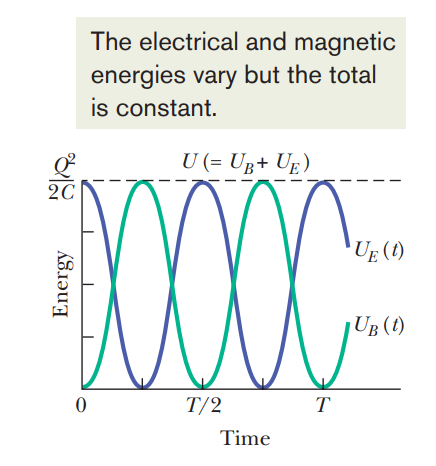
\includegraphics[width = 6cm]{Energy Oscillator.png}
    \caption{The Energy Oscillations}
\end{figure}
\subsection{Damped Oscillations in an RLC Circuit}
$$\begin{aligned}
    & \frac{dU}{dt}=Li\frac{di}{dt}+\frac qC\frac{dq}{dt}=-i^2R\\
    &\Rightarrow L\frac{d^2q}{dt^2}+R\frac{dq}{dt}+\frac1Cq=0\\
    &\Rightarrow q=Qe^{-t/\tau}\cos(\omega t+\phi)
    &\omega=\sqrt{\omega_0^2-(1/\tau)^2}\\
    &1/\tau=R/(2L)
    \end{aligned}$$
Forced oscillations in a series RLC circuit at a driving
angular frequency $\omega_d$
$$\varepsilon = \varepsilon_m \cos \omega_d t, \quad i = I \cos(\omega_d t + \phi) $$    
\subsection{Impendance}
Assume the potential difference across a circuit element (resistor, capacitor, and inductor) is
$$v(t)=\Re\left(\tilde{V}e^{i\omega_dt}\right),$$
and the current in the element is
$$i(t)=\Re\left(\tilde{l}e^{i\omega_dt}\right).$$
Define complex impendance as:
$$\tilde{Z}=Z\mathrm{e}^{i\phi}=\frac{\tilde{V}}{\tilde{I}}.$$
\begin{figure}[htbp]
    \centering
    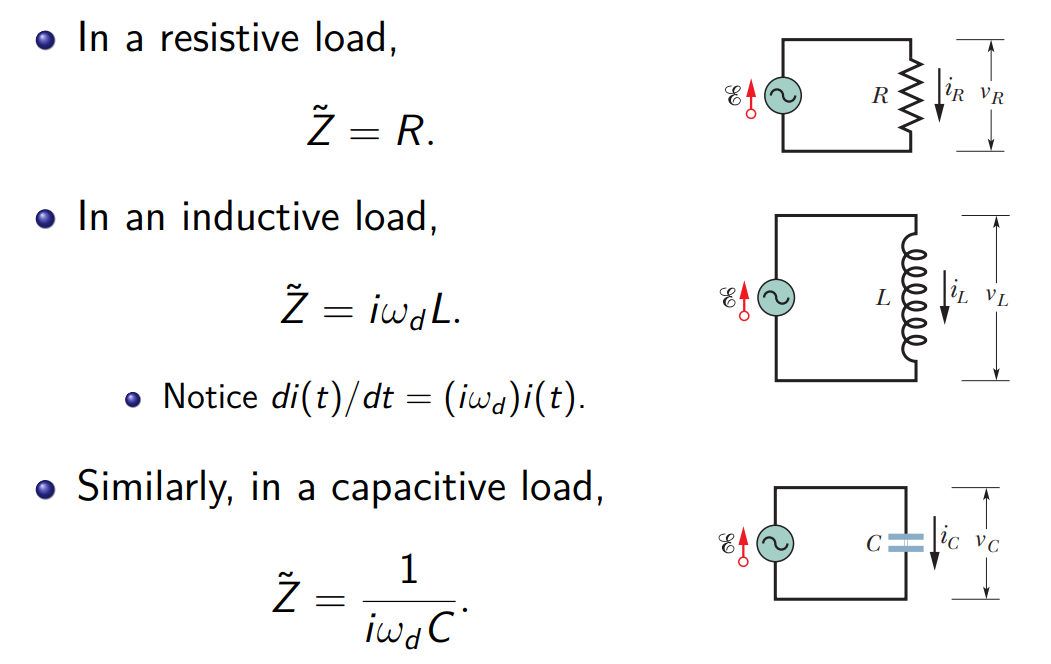
\includegraphics[width = 6cm]{Three Circuits.png}
    \caption{Three Circuits}   
\end{figure}
注意这里的$i$为虚数,$\Re$表示取实部

\section{Maxwell’s Equations and EM Waves}
\textbf{Maxwell's Equations}
Gauss's Law for $\vec{E}$:
$$\nabla \cdot \vec{E} = \frac{\rho}{\epsilon_0}$$
Faraday's Law:
$$\nabla \times \vec{E} = -\frac{\partial \vec{B}}{\partial t}$$
Gauss's Law for $\vec{B}$
$$\nabla \cdot \vec{B} = 0$$
Ampere-Maxwell's Law:
$$\nabla \times \vec{B} = \mu_0 \vec{J} + \mu_0 \epsilon_0 \frac{\partial \vec{E}}{\partial t}$$
In vacuum, electromagnetic waves satisfy:
$$\begin{aligned}\nabla^2\vec{E}&=\frac1{c^2}\frac{\partial^2\vec{E}}{\partial t^2}\\&\nabla^2\vec{B}=\frac1{c^2}\frac{\partial^2\vec{B}}{\partial t^2}.\end{aligned}$$

Therefore, in vacuum each Cartesian component of $E$ a $\vec{B}$ satisfies the wave equation
$$
\frac{\partial^2f}{\partial t^2}=c^2\nabla^2f,
$$
where the speed of all electromagnetic waves is
$c= \frac 1{\sqrt {\mu_0\epsilon_0}}\approx 3.00\times 10^8$m/s.
Electromagnetic waves are transverse:
$$
\hat{k}\cdot\vec{E}=\hat{k}\cdot\vec{B}=0.
$$
$\vec{E}$ is always perpendicular to $\vec{B}$:
$$
\vec{B}=\frac1c(\hat{k}\times\vec{E}).
$$
\end{document}